\chapter{Active knowledge extraction from cyclic voltammetry}\label{chapter3}
Cyclic Voltammetry~(CV) is an electro-chemical characterization technique used in an initial material screening for desired properties and to extract information about electro-chemical reactions.
In some applications, to extract kinetic information of the associated reactions (e.g., rate constants and turn over frequencies), CV curve should have a specific shape (for example an S-shape). 
However, often the settings to obtain such curve are not known \textit{a priori}. 
In this chapter, an active search framework is defined to accelerate identification of settings that enable knowledge extraction from CV experiments.
Towards this goal, a function space representation of CV responses is used in combination with Bayesian Model Selection (BMS) method to efficiently label the response to be either \textit{S-shape} or not \textit{S-shape}. 
Using an active search with BMS oracle, we report a linear target identification in a 6-dimensional design space (comprising of thermodynamic, mass transfer and solution variables as dimensions). 
The framework has the potential to be a powerful virtual screening technique for molecular catalysts, bi-functional fuel cell catalysts etc.


\section{Introduction}
Cyclic Voltammetry~(CV) is an electro-chemical characterization technique that measures current generated under a cyclic voltage load between a initial and final voltages varied at a given rate.
The measured current is a highly non-linear response from various physical phenomenon such as mass transport, kinetics, adsorption etc. 
In principle, it is possible to determine the properties associated with the underlying physical phenomenon. 
However, the property extraction is a non-trivial task. 
In a CV experiment, a steady state current is obtained when all reactions in the mechanism have the same apparent rate constants~\cite{BardFaulkner}. 
This is because the facile reactions in the sequence are held back from their maximum rates by the sluggish reactions called a \textit{rate determining step} that also determines the magnitude of steady state current.   
Extracting rate constants of the rate determining step thus requires the CV curve to be in a S-shape~\cite{costentin2015cyclic, rountree2014evaluation} with a clear steady state current region resolved during measurement. 
Towards this goal, obtaining a S-shaped CV curve requires the experiment to be run with a set of conditions~(e.g, temperature, substrate concentration, scan rate), amenable for S-shape CV curves which are unknown \textit{a priori}.
Moreover, choosing conditions where a given electrochemical system exhibits a S-shaped CV curve is dependent on underlying system of electrochemical reaction(s) which is(are) also unknown for novel materials. 
In the absence of a known mechanism, an exhaustive search over all the possible tunable parameters is performed~\cite{martin2016qualitative} to narrow down the region of interest. 
Such exhaustive strategy comes at a price of a very high computational cost especially in high-dimensional search spaces of multiple complex reaction mechanisms.

As an alternative approach, experts define a figure of merit~(FOM)~\cite{rountree2014evaluation}(a performance measure) as a proxy signature of a physical phenomenon of interest. 
FOM extracted from CV can be also used in material discovery using data-driven methods. 
For example, in~\cite{stein2019functional,li2019application,haber2014high,suram2015generating} different types of FOM have been used for catalyst discovery using data-driven methods.
With FOM defined, the goal is to find a material that produces a response with a FOM that is better than that of known materials.
For instance, in case of a high-throughput exploration for a new catalyst, the overpotential is a common FOM~\cite{norskov2004origin}(or performance measure) used in the combinatorial searches~\cite{suram2015generating}. 
The over-potential can be thought of as the voltage~(beyond the thermodynamic requirement) required to produce a (pre-defined) target current.
This FOM has clear utility to screen for well performing materials, but misses on the main advantage of CV - that is the capability to extract the kinetic information~(such as rate constants~\cite{FOWA}, turn-over frequencies~\cite{TOF,FOWA2}).

Given the time and financial constraints, an active learning method~\cite{jiang2018efficient,RGActiveIntro, GardnerALIntro} is proposed to accelerate the process of extracting kinetic information from CV curves. 
Rather than relying on the selection of figure of merit, a function space representation of our target~(S-shaped) and non-target~(everything else) CV responses is used in the Bayesian Model Selection (BMS) for automatic classification. 
We encode prior knowledge of target and non-target CV responses using the basis functions of a Gaussian processes~(\(\mathcal{GP}\)) function space.
\(\mathcal{GP}\) have been previously used to infer the kinetic parameters~\cite{gavaghan2018use,robinson2018separating} of a CV response by using a maximum likelihood estimate and \(\mathcal{GP}\) regression. 
In another work ~\cite{li2019application}, a Bayesian approach is used to search for an approximate rate constant when the reaction mechanism is known. 
In this work, however, \(\mathcal{GP}\) is used as a data representation model to distinguish S-shaped CV curves from other types of continuous CV curves. 
Once a S-shaped CV curve is collected, the foot-of-the-wave analysis~(FOWA)~\cite{FOWA} can be used to extract the rate constant of a rate determining step. 
When combined together with FOWA, the proposed approach can be a robust technique that does not require any knowledge of the actual reaction mechanism.

In this chapter, we focus on S-shaped CV responses due to their utility for:~a) extracting kinetic information~\cite{costentin2015cyclic, rountree2014evaluation}--using the foot of the wave analysis~\cite{FOWA} that can only be applied to a S-shaped CV curve.~b) screening for bi-functional catalysts -- materials that produce CV curves similar to S-shape in two different voltage sweep ranges~\cite{bradley2019reversible, jung2016optimizing}. 
While the two applications are different, they can be approached under a common framework of active search to find S-shaped CV curves within the combinatorial space. 


The rest of the chapter is organized as follows: (i)~First  Bayesian active learning framework is introduced with a general probabilistic model. Then a connection is established between collected data at observed locations with the oracle used to classify and update the decision model used for active learning. (ii)~Bayesian Model Selection~(BMS) procedure is then introduced to compute a classification preference for targets and non-targets based on collected data and a set of parametric models. (iii)~a \(\mathcal{GP}\) model is introduced from a function space representation point of view to be used as a parametric model in BMS.  (iv)~The methodology is then applied to a search space of a simple EC mechanism to demonstrate the application of the BMS oracle to classify CV responses in order of its S-shape. (v)~Finally, the BMS oracle is used in active search to address the challenges in knowledge extraction, virtual screening of materials for electrochemical applications using cyclic voltammetry.
\section{Methods}
The goal is to identify the measurement settings from which one can extract kinetic information captured in a CV response.
Towards this goal, we seek to identify measurement conditions for which an S-shape CV curve is collected by our oracle. 
We use an active learning technique summarized in~\Cref{fig:workflow} to accelerate the search for measurement settings within fixed computational budget. 
The active learning approach involves iterative collection of data points from a search space \(\mathcal{S}\).
The process starts with a small set of observed data \(D=(\textbf{S},\textbf{Y})\) where \(\textbf{S}\in\mathcal{S}\) are the observed locations and \(\textbf{Y}\in\{-1,1\}\) are corresponding labels. 
In each iteration, the algorithm collects data and incrementally updates the decision model \(p(y=+1|D)\) it aims to learn with \(y\) representing a label.
A user-defined selector~(or policy) identifies a~(or a batch of) candidate location(s) in the search space for observing the responses.
The policy typically maximizes a utility function given the decision model. 
For example, given \(D\), we can define a policy using a utility function that simply counts number of targets in the dataset \(u(\textbf{S})=\sum\limits_{s_i\in \textbf{S}, y_i \in \textbf{Y}} [y_i=+1]\). 
A policy can be defined to select more targets to be added to the data pool \(D\) using: 
\begin{equation}
    s^* = \argmax_s \mathbb{E}\left[ u(\mathcal{S} \setminus \textbf{S} | D )\right] 
    \label{eq:policy}
\end{equation}
Given a location \(s^* \in\mathcal{S}\), the corresponding experiment is performed and a response is collected. 
In this chapter, a CV response curve is collected from a CV curve simulator and the response is then passed onto an oracle. 
Oracle labels the response to be either a target or non-target~(for example in~\Cref{fig:workflow}, we show a non-target like CV shape which will be  assigned \(y^*=-1\) as a label). 
The next step is to augment \(D\) using the data collected in the current iteration i.e. \(D^* = D\cup (s^*,y^*) \). 
The decision model is then updated with \(D^*\). 
This process is repeated until computational budget--defined in terms of total number of label queries or equivalently number of simulations--is exhausted.
As an oracle we use a Bayesian Model Selection (BMS) that operates on two models \(\mathcal{M}_1, \mathcal{M}_2\) referred to as null model~(representing a typical CV curve) and target model~(representing an S-shaped CV curve), respectively.
Moreover, we use a variation of active learning called active search~\cite{garnett2012bayesian} which maximizes the number of targets found in contrast to traditional active learning where the selector is defined with a goal to closely approximate \(p(y=+1\vert D )\).


\begin{figure}[h]
    \centering
    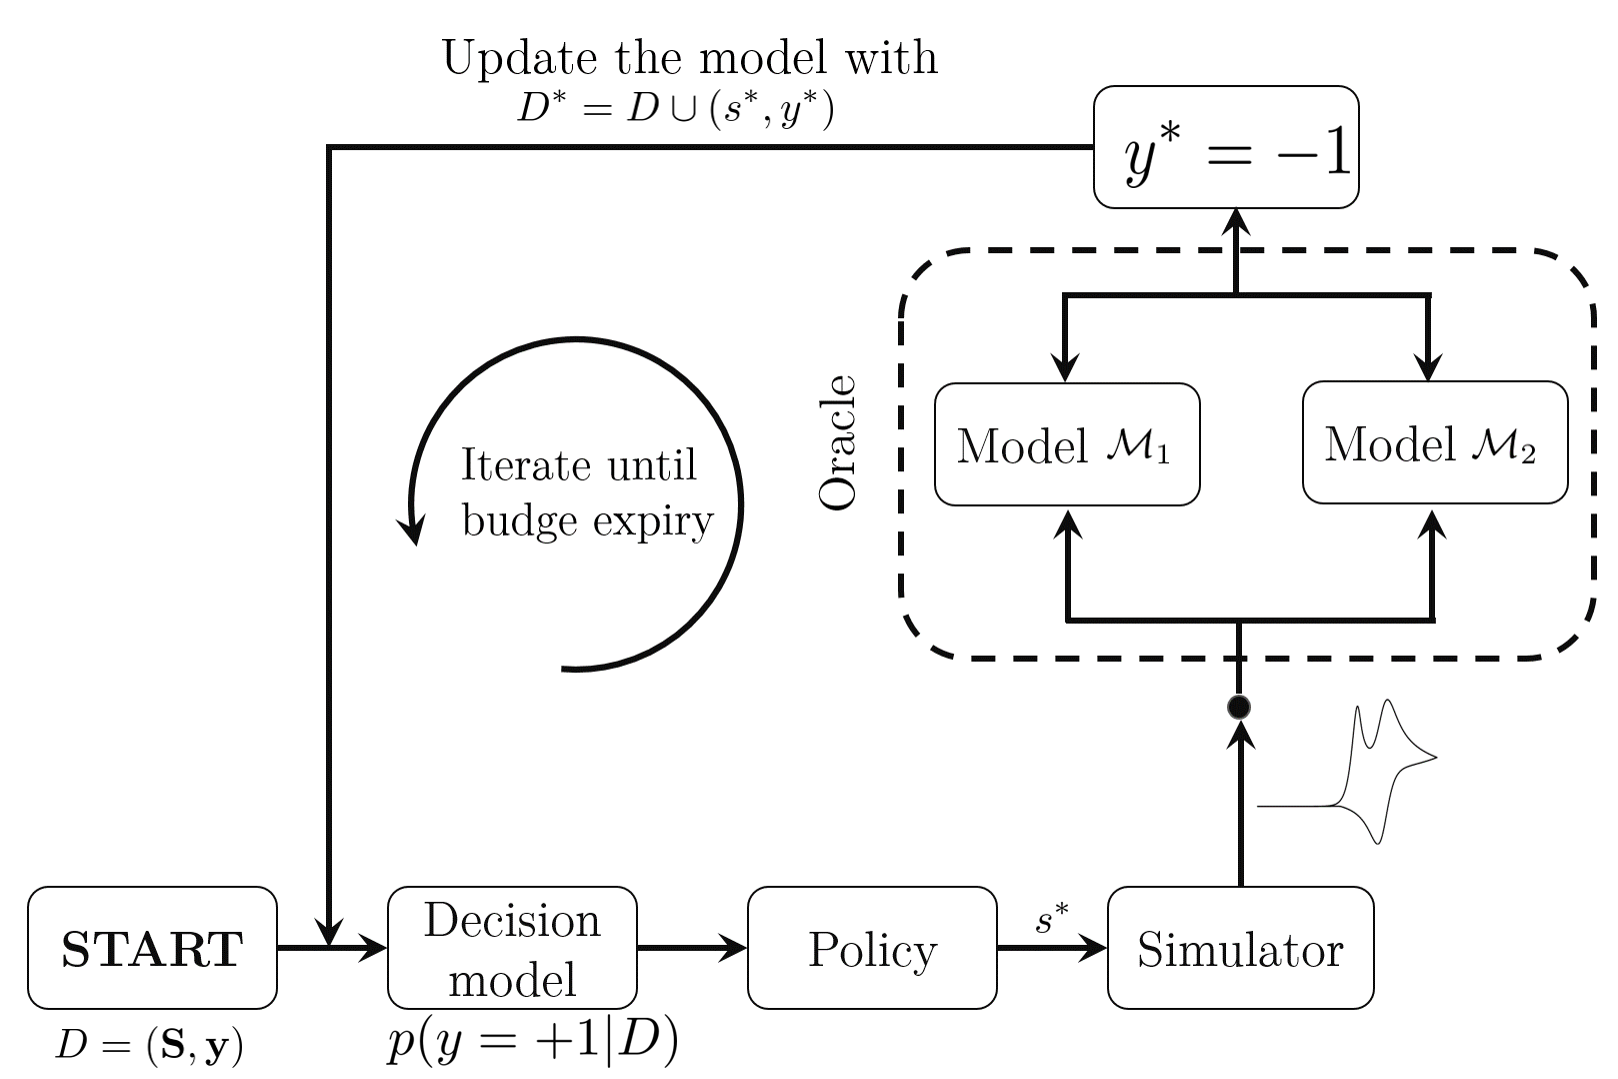
\includegraphics[width=0.75\linewidth]{Chapter-3/figures/workflow_gpcv.png}
    \caption{Active learning framework as a flowchart. Active learning iterations start with a few labelled data points in the search space \(\mathcal{S}\). We stop collecting data when we have selected a pre-defined number (called budget) of locations for updating our decision (or belief) model.}
    \label{fig:workflow}
\end{figure}

\section{Bayesian Model Selection}
The BMS is a tool to identify a preferred model from a family of parametric probability distributions, each of which can explain the observed data with differing degrees of fidelity. 
Using a supervised learning procedure that compares an input \(\textbf{X}\) and output \(\textbf{y}\), we compute a model posterior using Bayes rule to select the model that best explains the observed data \(\mathcal{D}=(\textbf{X},\textbf{y})\). 

Here, given the observed data \(\mathcal{D}=(\textbf{X}, \textbf{y})\), we compute probability that the data is sampled from any given model encoding our prior information. 
Computed posterior probabilities will be used as a score to differentiate whether the collected response (for example, a CV response at any input location in the search space of materials) is a target~(with higher probability for the corresponding target model) or not. 
In this chapter, we use both BMS and active learning in a related but different context. 
BMS is used with observed data encoding a single CV curve while active learning is used in the search space with their corresponding binary labels~(i.e. a target or not) as observed data. 
Moreover, BMS is used as an oracle for the active learning task with models \(\mathcal{M}_j\) as \(\mathcal{GP}\).

For each model \(\mathcal{M}\) with a parameter index \(\theta\)-- a concatenated vector of hyper-parameters-- we first compute model evidence \(p(\textbf{y}\vert \textbf{X},\mathcal{M})\) on the observed data \(\mathcal{D}=(\textbf{X}, \textbf{y})\):
\begin{equation}
    p(\textbf{y}\vert \textbf{X},\mathcal{M}) = \int p(\textbf{y}\vert \textbf{X},\theta,\mathcal{M})p(\theta\vert \mathcal{M}) \diff \theta
\label{eq:evidM}
\end{equation}
where \(p(\textbf{y}\vert \textbf{X},\theta,\mathcal{M})\) is probability of obtaining outputs \(\textbf{y}\) given input data \(\textbf{X}\) and a model \(\mathcal{M}\). \(p(\theta\vert \mathcal{M})\) represents distribution of parameter \(\theta\) for any given model \(\mathcal{M}\).

To understand which model to prefer from a finite set of models  \(\bigl\{\mathcal{M}_i\bigr\}_{i=1}^n\), we apply the Bayes rule to compute the posterior probability of each model \(\mathcal{M}_{j}(j\in\{1,2,..n\})\) given data \(\mathcal{D}\) using the posterior of~\Cref{eq:evidM}: 
\begin{equation}
    p(\mathcal{M}_j\vert \mathcal{D}) = \frac{p(\textbf{y}\vert \textbf{X},\mathcal{M}_j)p(\mathcal{M})}{p(\textbf{y},\textbf{X})}
    \label{eq:postM}
\end{equation}
where \(p(\mathcal{M})\) represents a prior over the finite set of models that is typically taken to be uniform i.e. no prior preference to any single model. 
One common approach is to use logarithm of the probability which can be interpreted as the information content of a probability model given data. 
Taking the logarithm of~\Cref{eq:postM}, we get the following~(See Supplementary Information): 
\begin{equation}
    \log p(\mathcal{M}_j\vert \mathcal{D}) = -\log \left [ 1+\sum_{i\neq j}^{n} \frac{p(\textbf{y}\vert \textbf{X},\mathcal{M}_i)}{p(\textbf{y}\vert \textbf{X},\mathcal{M}_j)}\right]
\label{eq:logPostM}
\end{equation}





\subsection{\(\mathcal{GP}\) Models for Catalytic Responses}
A \(\mathcal{GP}\) is a distribution over smooth latent functions \(g: \mathcal{X} \rightarrow \mathbb{R}\). 
Assuming the observation model \(p(y\vert g)\) is known, the standard approach is to use non-parametric Bayesian approach by placing a \(\mathcal{GP}\) distribution over \(g\), i.e. \(p(g)=\mathcal{GP}\big(\mu(x),k(x,x')\big)\). 
Here \(\mu(x):\mathcal{X}\rightarrow \mathbb{R}\) is a mean function and \(k(x,x'):\mathcal{X}\times\mathcal{X}\rightarrow \mathbb{R}\) is a covariance function. 
A function-space viewpoint provides an intuitive explanation of \(\mathcal{GP}\) as vector space of functions in a chosen (potentially non-linear) feature space which \(\phi(x)\) as a basis. 
In the function space representation, the observation model plays the role of weights \(W\) with function \(g\) represented using \(g(x) = \phi(x)^{\top}W\). 
It can be shown~(see Supplementary Information) that \(\phi(x)\) can be implicitly defined using the covariance function \(k(x,x')\) between pair of inputs \(x,x'\in\mathcal{X}\) and a mean function \(\mu(x)\) of \(W\)~\footnote{for this reason we use \(k(x,x')\) and basis function of \(\mathcal{GP}\) interchangeably in this paper}. 
The mean function \(\mu\) encodes an average behavior of the function \(g\). 
The covariance function \(k(x,x')\) encodes the correlations between outputs \(g(x), g(x')\) for any given pair of input points~(\(x,x'\)). 
In this chapter, the concatenated vector of the parameters \(\mu(x)\) and \(k(x,x')\) is denoted as \(\theta\).
Once we select a \(\mathcal{GP}\) encoding our prior beliefs, we use Bayes rule to update our posterior \(p(g\vert \mathcal{D})\) conditioned on observed data \(\mathcal{D}=(\textbf{X},\textbf{y})\) where \(\textbf{y}\) are the discrete evaluations of function \(g\) at inputs \(\textbf{X}\). 
For more information on \(\mathcal{GP}\), readers are referred to~\cite{williams2006gaussian}.

A typical response from a cyclic voltammetry experiment is represented as a function \(I(t,v)\) with \(I\) being the current response collected at a time (\(t\)) for a time dependent applied voltage \(v=V(t)\). 
The voltage load \(V(t)\) is typically chosen to be linear and the voltammetry is often referred as direct current voltammetry~\cite{li2019application}.
Classification of a CV into an S-shape (or not S-shape) can be looked at as determining a model evidence of a function defined by CV curve \( (v,t) \mapsto I\) under a \(\mathcal{GP}\) function space with observed data \(\mathcal{D}\) given by the discrete CV curve \(\textbf{X} = I, \textbf{y}=(v,t)\). 
The covariance of a CV curve gives rise to the basis functions in the \(\mathcal{GP}\) space and the time-voltage grid becomes the input space where the function is evaluated.
For any given CV curve, its representation in the \(\mathcal{GP}\) function space  is obtained by finding a \(\theta\) that maximize the posterior probability \(p(\textbf{X} = I|\textbf{y}=(v,t))\)~\footnote{we use the \textit{maximum a posteriori} or MAP estimation}.
The \(\mathcal{GP}\) model is chosen with a \textit{non-stationary} covariance as a target model~\(\mathcal{M}_2\). 
It follows from the reproducing kernel Hilbert space~(RKHS) theorem~(Ch 12.4 in \cite{mathML}) that any smooth function can be represented using a kernel or a covariance function.
Thus for the null model~(\(\mathcal{M}_1\)), it is sufficient to use a \(\mathcal{GP}\) with smoothness controllable covariance function. 
A brief overview of the covariance functions selected as basis functions is described below.
For both models \(\mathcal{M}_1\) and \(\mathcal{M}_2\), the mean function is chosen to be \(\mu(x)=0 \) as we normalize the response curves \(I(v,t)\) to be with in \((0,1)\) and expect the covariance function to determine the shape of the CV curve. 

\subsubsection{Squared Exponential Covariance}
The commonly known \textit{squared exponential kernel}~(in~\Cref{eq:covSEard} and~\Cref{fig:covSEard}) is used as a covariance model for \(\mathcal{M}_1\) where the resulting feature map \(\phi(x)\) forms a basis for functions that are smooth and stationary.
\begin{equation}
    k(x,x')=\sigma_f^2 \exp((x-x')^{\top}\Lambda^{-1}(x-x'))
    \label{eq:covSEard}
\end{equation}
In~\Cref{eq:covSEard}, \(\sigma_f\) is scaling parameter, and \(\Lambda\) is a diagonal matrix with each entry as a length scale for the corresponding dimension of \(x,x'\in \mathcal{X}\). 
The left panel of \Cref{fig:covSEard} depicts five samples drawn at random from the \(\mathcal{GP}\) with the covariance in~\Cref{eq:covSEard}.% The input to the function \(g\) s \(x\) and real valued outputs as \(g(x)\). 
The right panel of the same figure depicts the covariance function visualized on a uniform grid of \(\mathcal{X}\times\mathcal{X}\) as contours. 
From~\Cref{fig:covSEard}, it can be seen that the covariance is stronger~(\(\approx 1\)) between inputs with Euclidean norm~(i.e. distance) less than a length scale controlled by the parameter \(\Lambda\).

\begin{figure}[h]
    \centering
    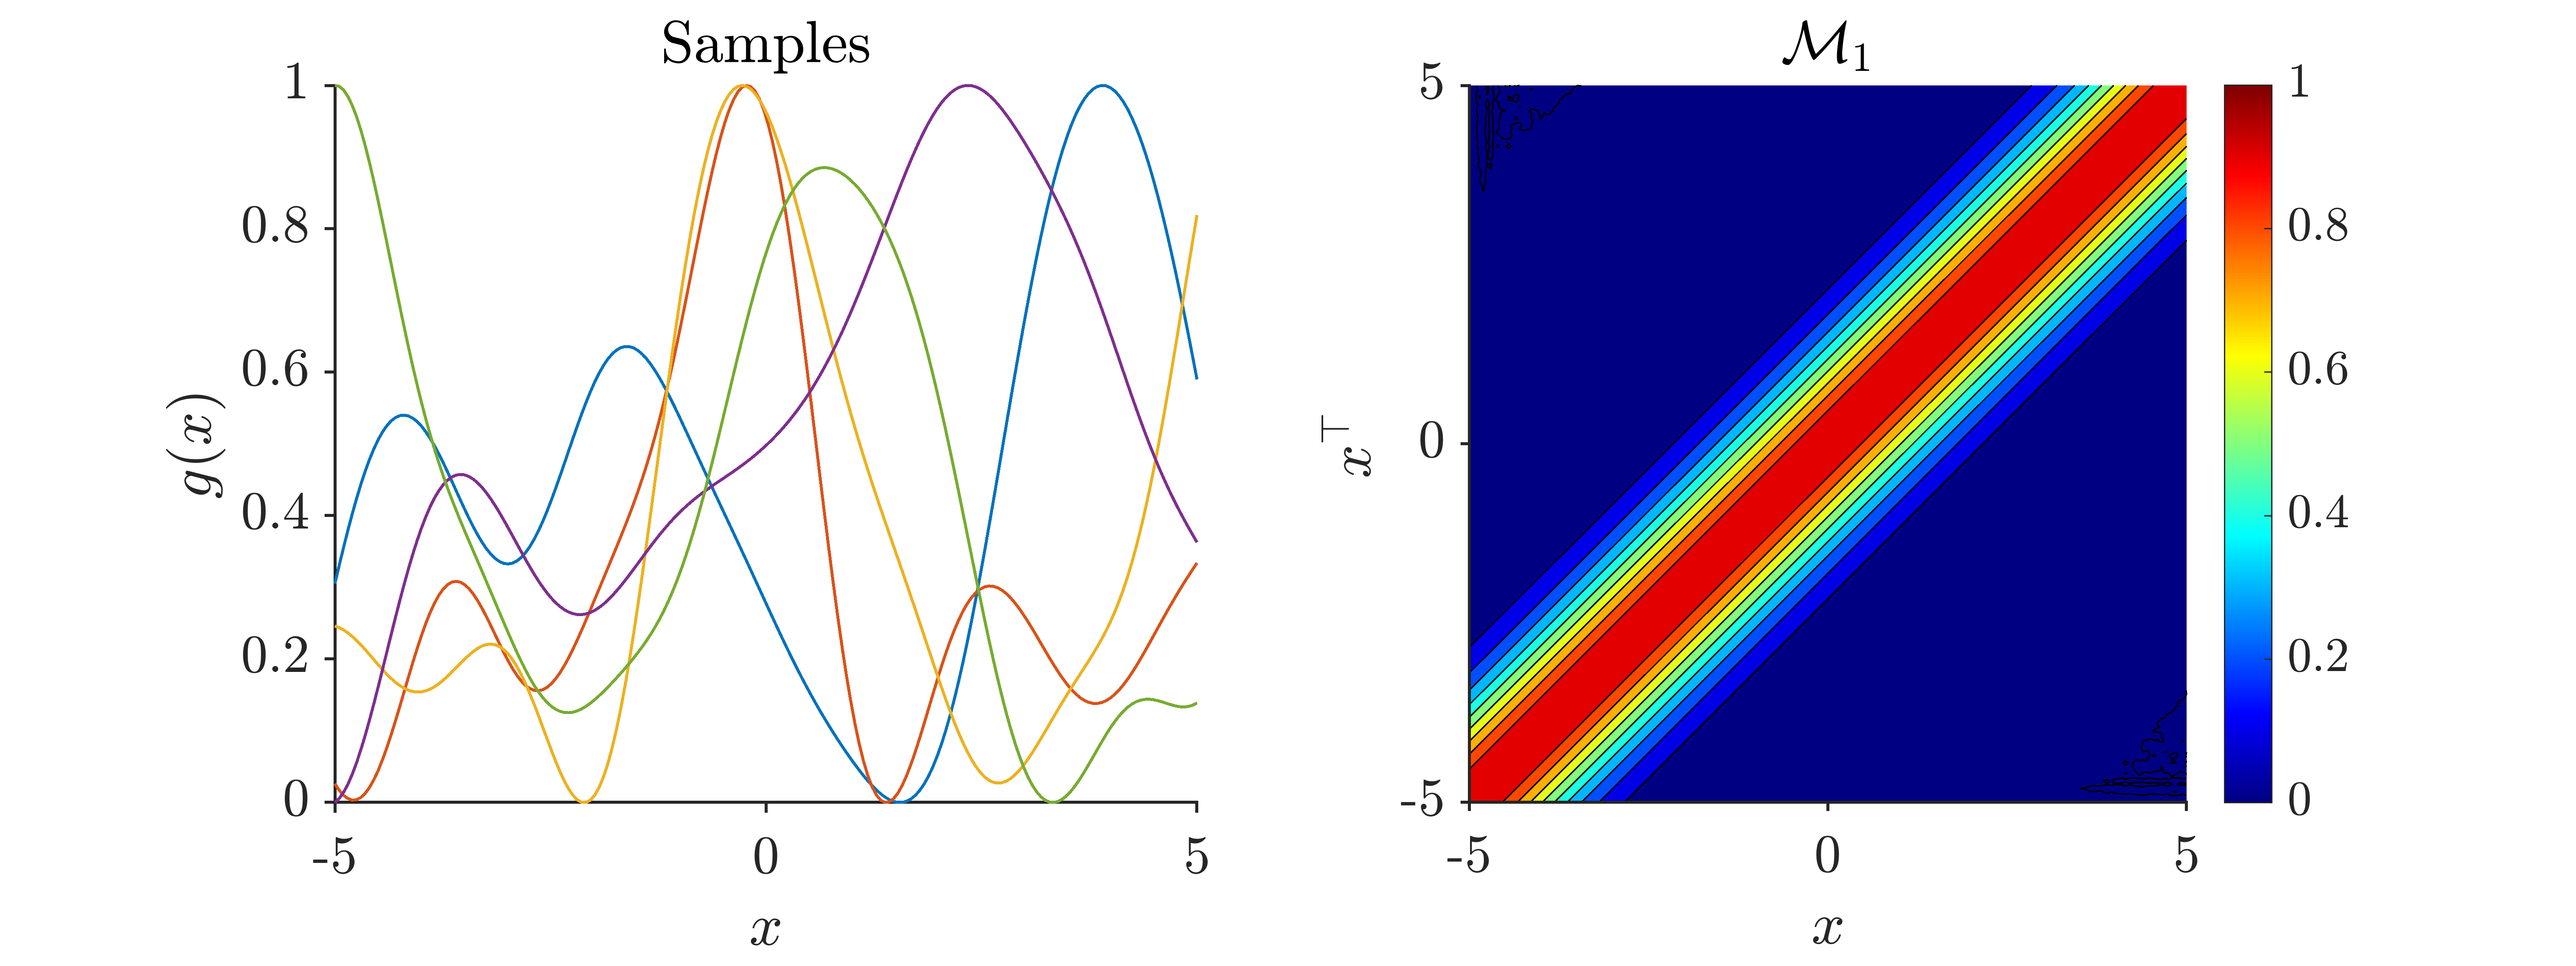
\includegraphics[scale=0.5]{Chapter-3/figures/Model1.png}
    \caption{A pictorial representation of~\Cref{eq:covSEard}. Left panel: five samples drawn at random from the \(\mathcal{GP}\) built using~\Cref{eq:covSEard}, captures the smooth and locally correlated nature of the \(\mathcal{GP}\). Right panel: a contour plot depicting correlations between outputs of one-dimensional vectors \(x,x' \in \mathcal{X}\). Color code represents the covariance \(k(x,x')\) with red representing high covariance i.e. output values \(g(x), g(x')\) are highly correlated and vice-versa. }
    \label{fig:covSEard}
\end{figure}

\subsubsection{Neural Network Covariance}
The target model uses neural network covariance kernel to build a \(\mathcal{GP}\) function space representation referred as model~\(\mathcal{M}_2\)(shown in~\Cref{eq:covNNone} and~\Cref{fig:covNNone}).
The S-shape responses have a non-stationary covariance and hence a covariance that is effective in handling rapidly changing signals would be a good choice. 

\begin{align}
        k(x,x') &= \sigma_f^2 \sin^{-1}\left({\frac{x^{\top}\Lambda^{-2}x'}{\sqrt{h(x)h(x')}}}\right) \label{eq:covNNone}\\
        h(x) &= 1+x^{\top}\Lambda^{-2}x \nonumber
\end{align}
In~\Cref{eq:covNNone}, \(\sigma_f\) is scaling parameter, and \(\Lambda\) is a diagonal matrix with each entry as a length scale.
\Cref{fig:covNNone} is analogues to~\Cref{fig:covSEard} and it can be seen that the covariance is high~(\(\approx 1\)) in two blocks of input locations that are separated by a completely uncorrelated input locations~(covariance \(\approx 0\)). 
This is in contrast to \(\mathcal{M}_1\) where the covariance is determined by some form of distance between input points. 
\begin{figure}[h]
    \centering
    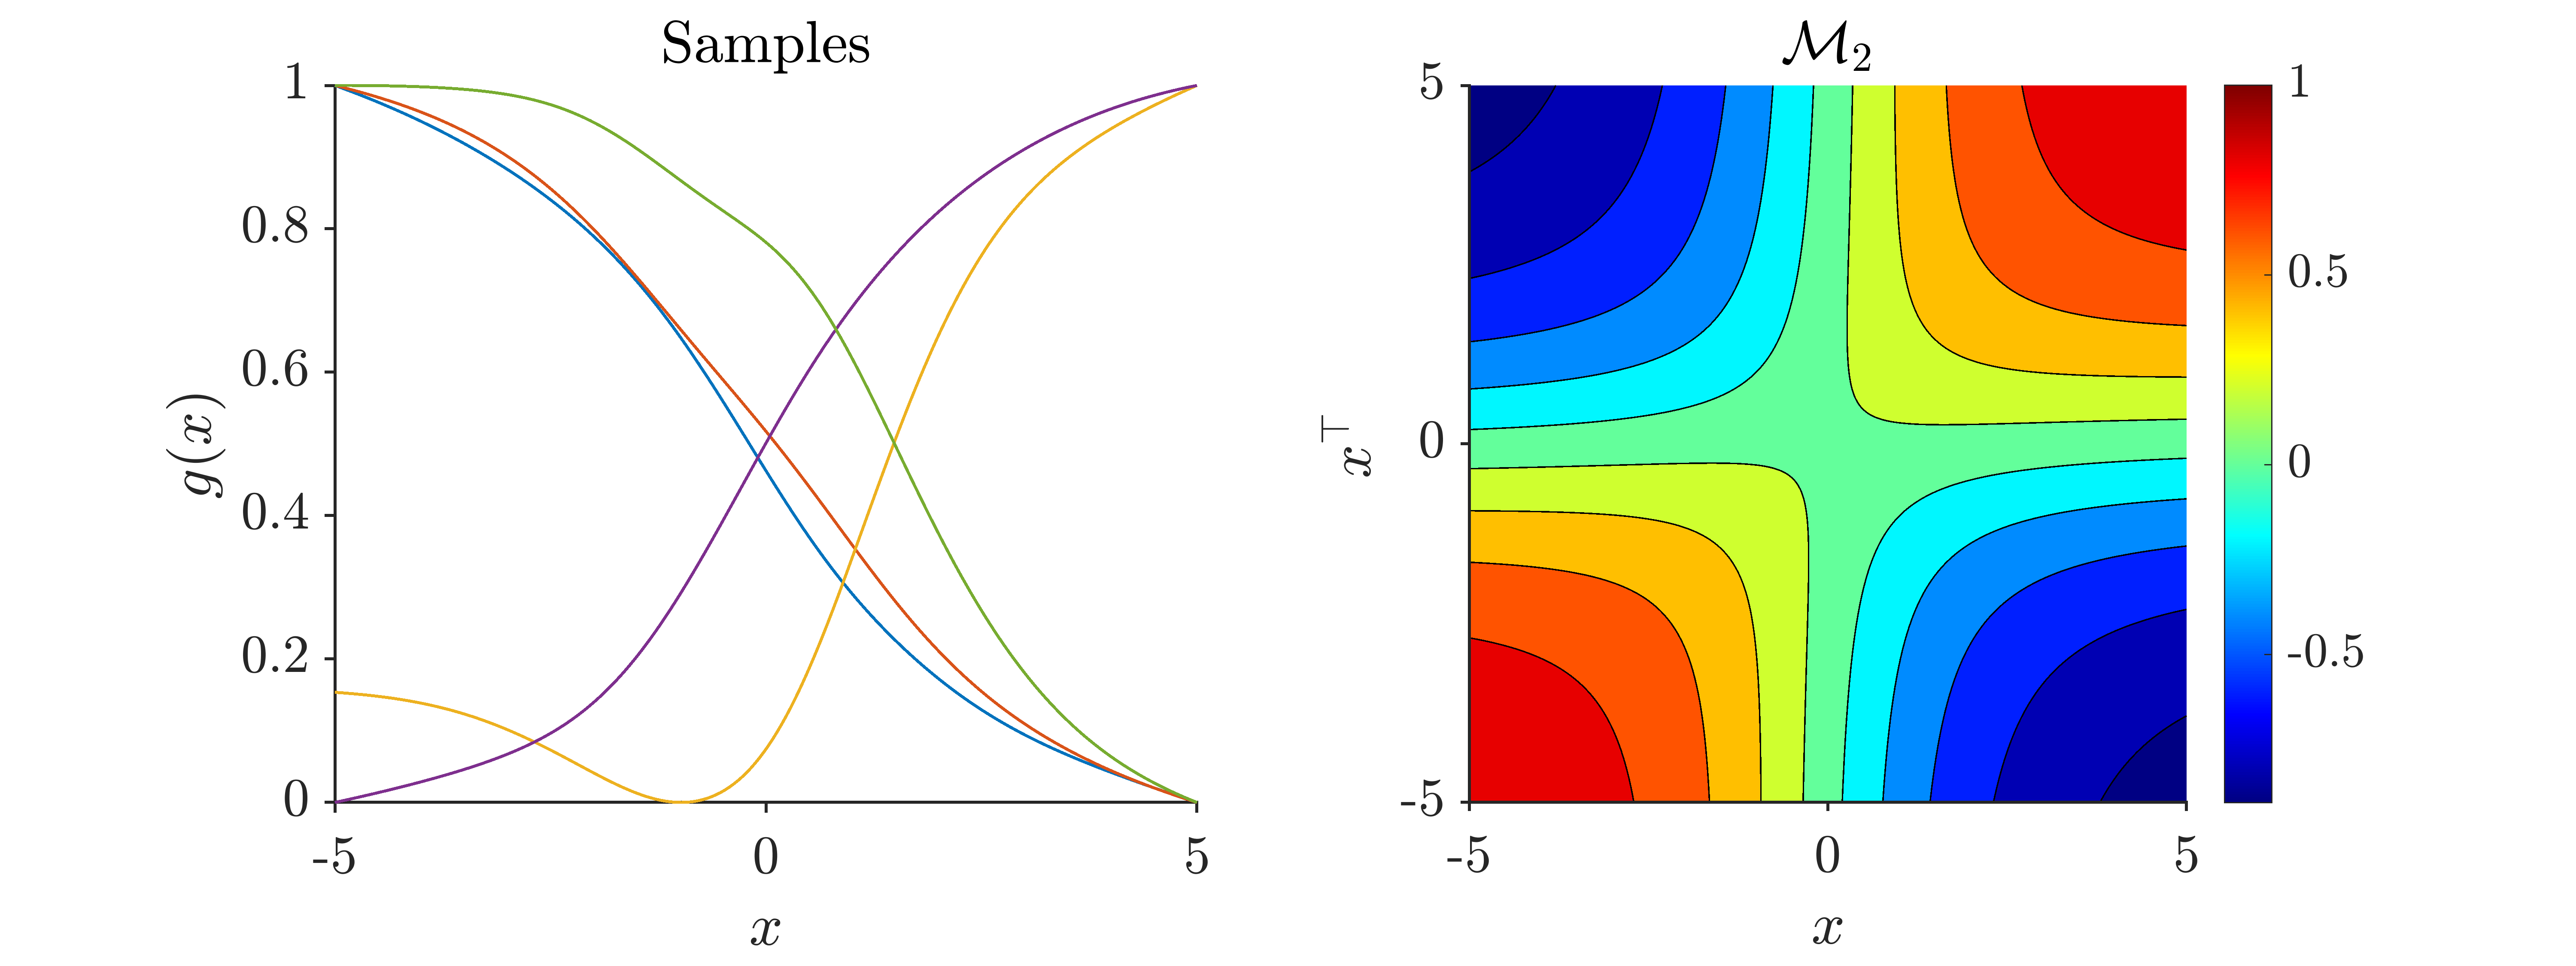
\includegraphics[scale=0.5]{Chapter-3/figures/Model2.png}
    \caption{A pictorial representation of~\Cref{eq:covNNone}. Left panel: five samples drawn at random from the \(\mathcal{GP}\) built using~\Cref{eq:covNNone}, captures the non-stationary nature nature of the \(\mathcal{GP}\) signified by constant values and sharp rises in the response values. Right panel: a contour plot of covariance between two one-dimensional vectors \(x,x' \in \textbf{X}\) as inputs. A positive value for \(k(x,x')\) signifies that output values \(g(x), g(x')\) are highly correlated and vice-versa. }
    \label{fig:covNNone}
\end{figure}



\section{Results}
To demonstrate the application of active search for S-shaped CV curves, we choose to simulate CV curves of a classic EC-mechanism, that consists of two reactions: E and C (\Cref{E} and \Cref{C}) corresponding to one electron transfer reaction (E) and one chemical reaction (C), respectively. 
EC-mechanism is selected as it is a well studied mechanism~\cite{rountree2014evaluation, costentin2015cyclic} that produces a variety of CV shapes thus serves as a good test case for the oracle described earlier. 
In this work, we use the MECSim simulator~\cite{MECSim} to generate CV curves on demand. 

\subsection{Data generation}\label{sec:data}
The EC mechanism is a two step reaction comprising of an electron transfer~\Cref{E} followed by a chemical reaction in~\Cref{C}. 
\begin{chequation}
\begin{align}
    &\ce{P + e <=> Q} \label{E}\\
    &\ce{Q + A -> P } \label{C}
\end{align}
\end{chequation} 
Electro-chemical kinetics of the EC mechanism can be modeled and solved using governing partial differential equations~\cite{saveant1984homogeneous}. 
In this section, we are interested in modeling the (micro)kinetics of species (and electron) that contributes to current generation under cyclic voltage sweep at a given sweeping rate.

Towards this goal, the transport of the three species (P, Q, A) in the solution is modelled using Fick's second law of diffusion with a source term corresponding to the heterogeneous reactions:
\begin{align}
    \pdv{C_P}{t} &= D_{\text{diff}}\pdv[2]{C_P}{u} + k_{s}C_{Q}C_{A} \nonumber\\
    \pdv{C_Q}{t} &= D_{\text{diff}}\pdv[2]{C_Q}{u} - k_{s}C_{Q}C_{A} \nonumber\\
    \pdv{C_A}{t} &= D_{\text{diff}}\pdv[2]{C_A}{u} - k_{s}C_{Q}C_{A} \label{eq:fickslaws}
\end{align}
with the boundary conditions defined as follows:
\begin{align}
    t&=0, \forall u &  &C_P = C^0_{P}, C_A = C^0_{A}, C_Q = C^0_{Q} \nonumber \\
    t&>0, u\rightarrow \infty &  &C_P = C^0_{P}, C_A = C^0_{A}, C_Q = C^0_{Q}  \nonumber\\
    t&>0, \forall u &  &\pdv{C_A}{u}=0; \pdv{C_P}{u}+\pdv{C_Q}{u}=0; C_P/C_Q = \exp(\frac{F}{RT}(V-E^0)) \label{eq:bcs}
\end{align}
In~\Cref{eq:fickslaws,eq:bcs} the formal reversible potential of electron transfer reaction~\cref{E} is \(E^0\), the  concentration of catalyst P is \(C_P\), specie Q is \(C_Q\) and substrate A is \(C_A\). \(D_{\text{diff}}\) is a common diffusion coefficient for all species and \(k_{s}\) is the rate constant of the forward reaction in~\Cref{C}. 
The spatial domain is denoted as \(u\) starting from the working electrode~(i.e. \(u=0\)) assuming a semi-infinite domain. The time scale of the simulation is denoted as \(t\). Initial concentrations~(i.e. at \(t=0\)) are denoted with a superscript 0. \(V\) represents the time varying applied voltage. 
For a cyclic voltage sweep between voltages \(V_i, V_f\) at a rate of \(\nu~V/s\) we get~\Cref{eq:voltage_scan} for V~(\(T_s\) is switching time).
\begin{align}\label{eq:voltage_scan}
    V(t) = 
    \begin{cases}
        V_i + \nu t & 0<t<T_s\\
        V_f - \nu t & T<t<2T_s
    \end{cases}
\end{align}
Digital simulation of system of partial differential equations in~\Cref{eq:fickslaws,eq:bcs} is performed to determine spatio-temporal concentration profiles of species P, Q, A. 
The Faradaic current observed during the cyclic voltage load is computed using~\Cref{eq:current} following the Butler-Volmer model for heterogeneous electron transfer at the electrode surface.
\begin{align}\label{eq:current}
    i(t,v) = FA_{\text{surf}}k^0\left[C_Q\exp(\frac{\alpha F}{RT}(V-E^0)) - C_P\exp(\frac{(1-\alpha)F}{RT}(V-E^0))\right]
\end{align}
In~\Cref{eq:current}, \(F\) is Faraday's constant, \(A_{\text{surf}}\) is surface area of electrode~( \(=1~cm^2\)), \(R\) is universal gas constant, \(T\) is room temperature.
\(k^0\) is heterogeneous electron transfer rate constant and \(\alpha\) is a symmetric charge transfer coefficient~(=0.5).
    
We use the freeware software MECSim~\cite{kennedy2015monash,MECSim} to digitally simulate the cyclic voltammetry response in the voltage range of \([-0.5V,0.5V]\). 
Along with the parameters used in~\Cref{eq:fickslaws,eq:bcs}, MECSim can also simulate the effects of an uncompensated resistance (\(R_u\)), double layer capacitance (\(C_{dl}\)) which are not used in this example case study. 
We form a 6-dimensional design search space using \(C_P^0, C^A_0, k_{s}, k^0, \nu, E^0\) and set the values of \(R_u = 0, C_{dl} = 0, \alpha=0.5, D=1\times10^{-5}\). 
\Cref{tab:search_space} lists the combinatorial space defined with six design variables (dimensions of search space) and number of samples along the dimension used to create an exhaustive search grid of tunable settings.
After excluding responses from a diverging simulation arising from a combination of non-physical parameters for MECSim~\footnote{see MECSim documentation for known limitations} we get a total of \(\approx 17\times10^3\) CV curves in our database. 
\begin{table}[h]
\centering
\begin{tabular}{|c|c|c|}
\hline
Parameter & range & number of levels per dimension \\  \hline
\(\log C_P^0 \) &[-2,3] & 5\\ \hline
\(\log C_A^0 \) &[-2,3] & 5\\ \hline
\( E^0 \) &[-0.4,0.4] & 5\\ \hline
\(\log k_{s} \) &[-1,6] & 5\\ \hline
\(\log k^0 \) &[-1,6] & 5\\ \hline
\(\log \nu \) &[-2,4] & 6\\ \hline
\end{tabular}
     \caption{Combinatorial space used to generate CV responses in EC mechanism along with number of levels used in the exhaustive search.}
     \label{tab:search_space}
 \end{table}
 


\subsection{Using BMS as an oracle to identify S-shaped CV curves}
The application of the BMS oracle to label the CV responses as target, if they are of S-shape, and as non-targets otherwise is demonstrated in this section. 
The proposed BMS oracle is used to label the CV responses and couple it with standard active search techniques to find our "targets" within a given budget of label queries (equivalently number of queries to the simulator). 
To accommodate for the high-throughput search running a batch of experiments at a time, we run the active search using both sequential selection of query locations~(batch size \(b=1\)) and a batch selection~(\(b=100\)). 
We use the  design space in~\Cref{tab:search_space} and aim to find as many targets as possible in the resulting combinatorial design space~\(\mathcal{S}\) of six parameters (dimension of \(\mathcal{S}\)). 

To demonstrate the efficacy of the proposed methods, we first pre-compute labels for a set of ten CV curves in \(\mathcal{S}\) of varying shape.
\Cref{fig:repbmsscores} depicts the chosen CV curves ordered based on model posterior~(\Cref{eq:logPostM}) percentile rank.
Notably, the highest scored CV curves have the S-shape which are of interest in this work.
From~\Cref{fig:repbmsscores}, it can be noted that BMS assigned the highest score to CV curves where the forward and backward sweeps overlap exactly i.e. no hysteresis or capacitive behavior~(highlighted using a red box). 
On the other spectrum, the oracle labels several types of CV curves with low scores.  

The good performance of BMS in this study can be attributed to its inherent ability to handle Gaussian noise, which is also of practical interest for cyclic voltammetry responses~\cite{gavaghan2018use}. 
For comparison, we studied two other oracles to rank a CV curve based on their S-shape characteristics using point-wise comparison: a)~\textit{similarity score} that uses a generic approach of computing the Euclidean norm between a given CV curve and user defined reference S-shape; and b) \textit{FOWA score} that is physics inspired and defined as the \(R^2\)-value for any CV curve in Foot of The Wave Analysis~(FOWA) coordinate space~(a perfect symmetric S-shaped CV curve has \(R^2=1\)). 
% We discuss more details on (a,b) in Supplementary Information. 
\begin{figure}[h]
    \centering
    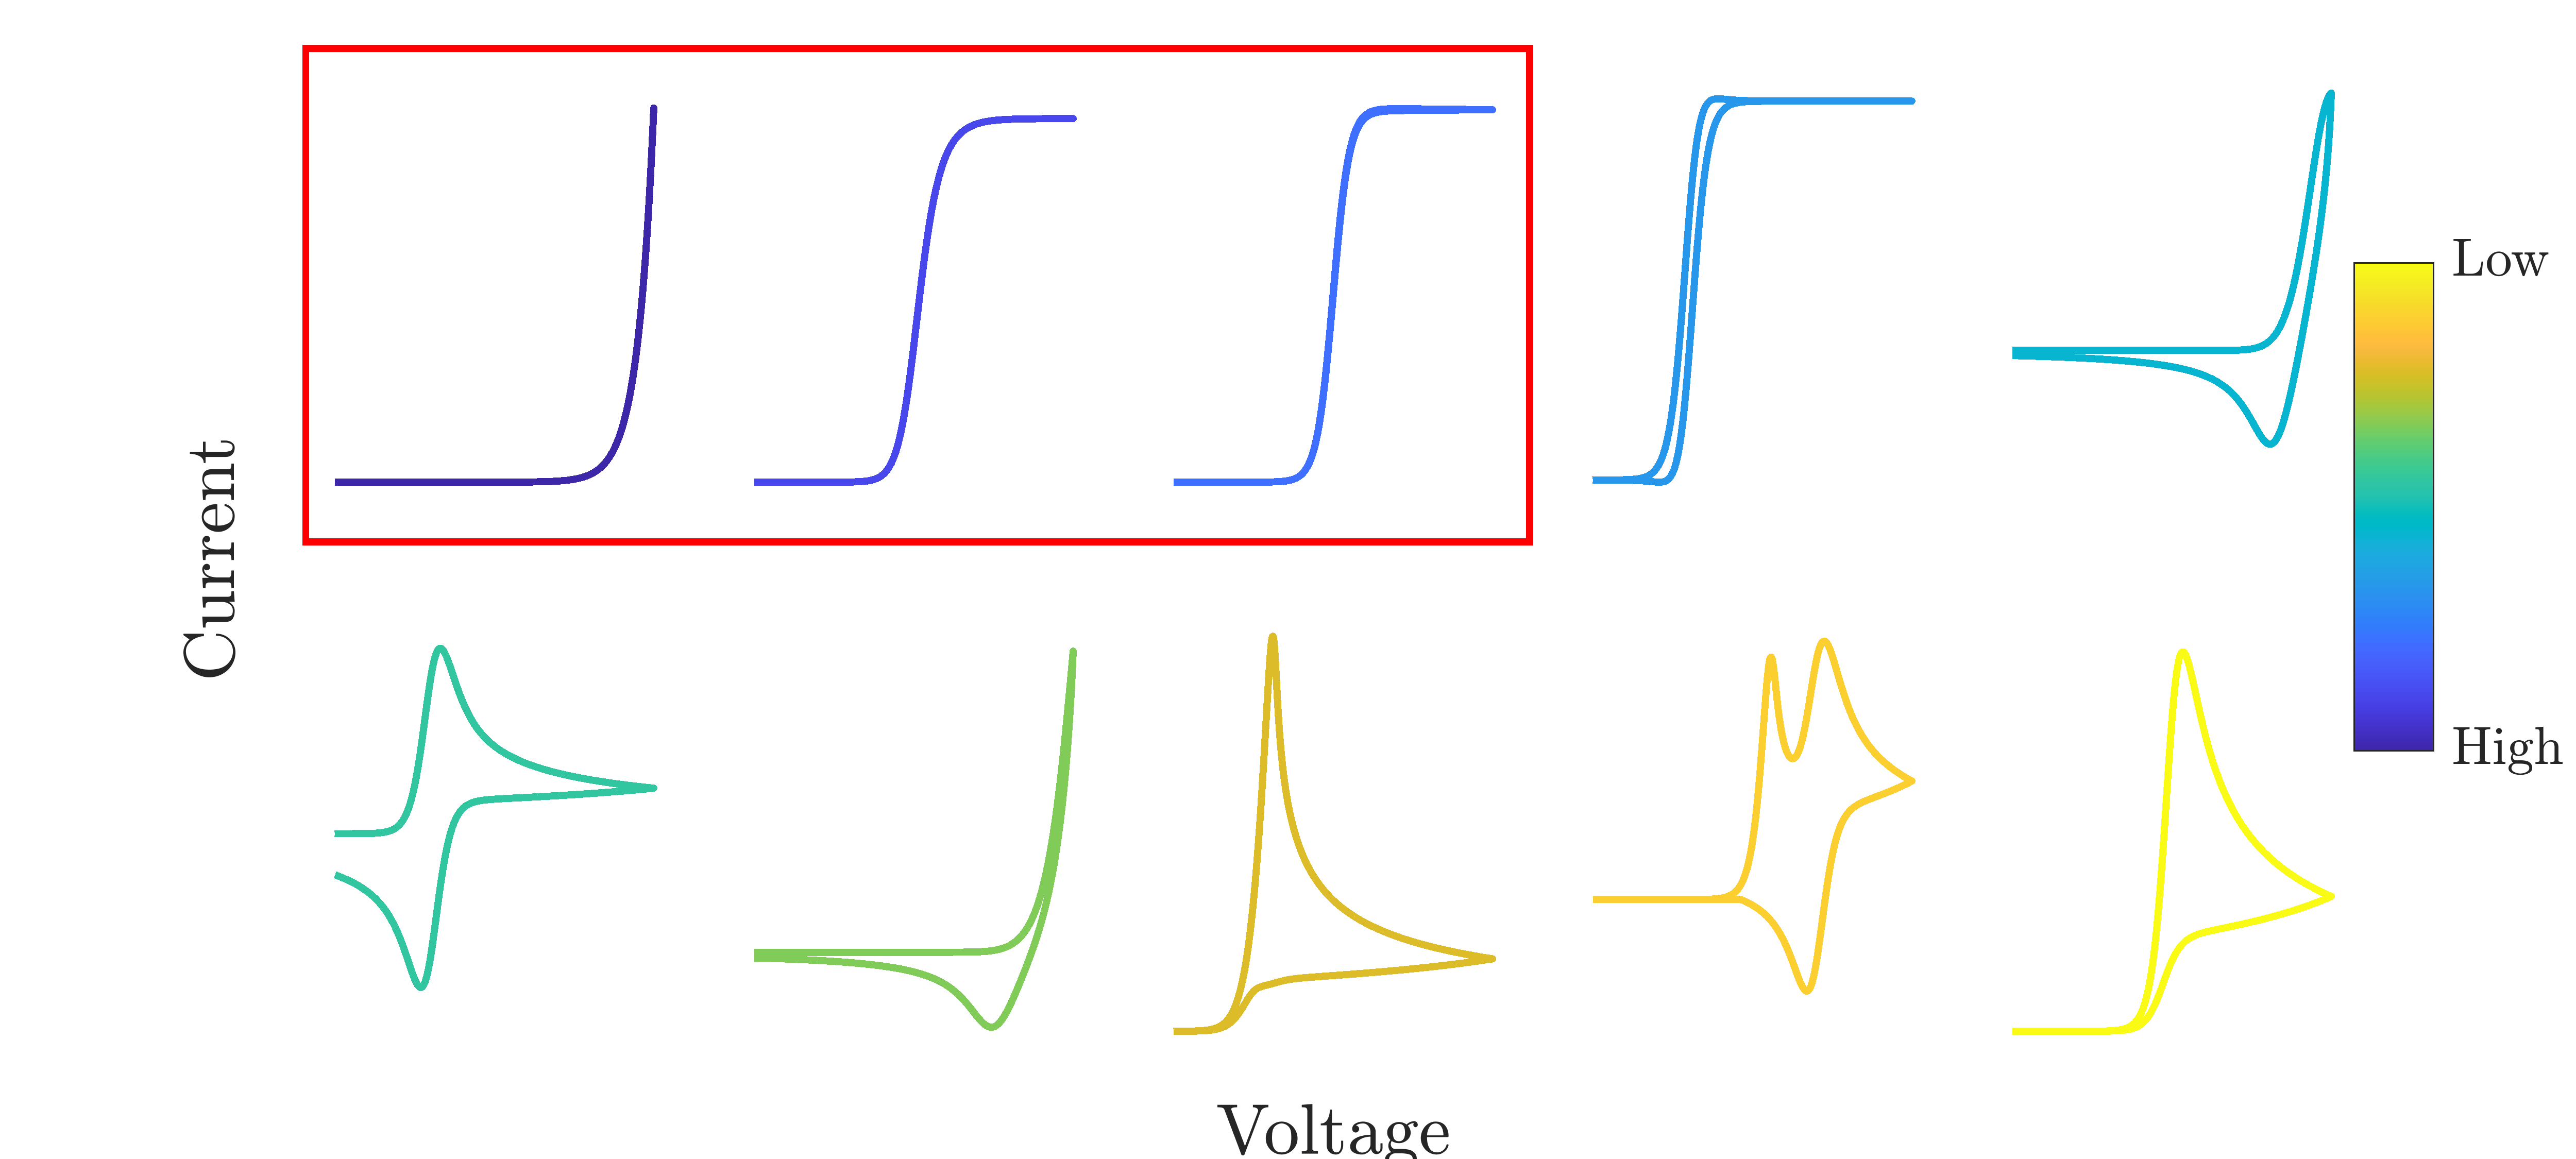
\includegraphics[width=100mm]{Chapter-3/figures/repbmsspectrum.png}
    \caption{Representative CV curves from the dataset ordered and color coded using the BMS score. CV curves boxed in red will be labelled as targets by the oracle.}
    \label{fig:repbmsscores}
\end{figure}

\subsubsection{Similarity score based oracle}
A Euclidean norm between a reference CV curve \(I_{ref}\) and any given CV curve \(I\) is computed using \(\sum \sqrt{(I - I_{ref})^2}\) both represented as vectors in a high-dimensional space and sum taken over the components. 
In~\Cref{figSI:repssscores} ten representative CV curves are depicted by sorting and color-coding based on the similarity score (similar to~\Cref{fig:repbmsscores}). 
The results showcase poor performance of the similarity score and ordering the CV curves with only two targets in the top three.
Although it marks the first curve correctly with high score, it fails to identify other S-shaped curve that is shifted along the voltage with respect to the first curve.
\begin{figure}[h]
    \centering
    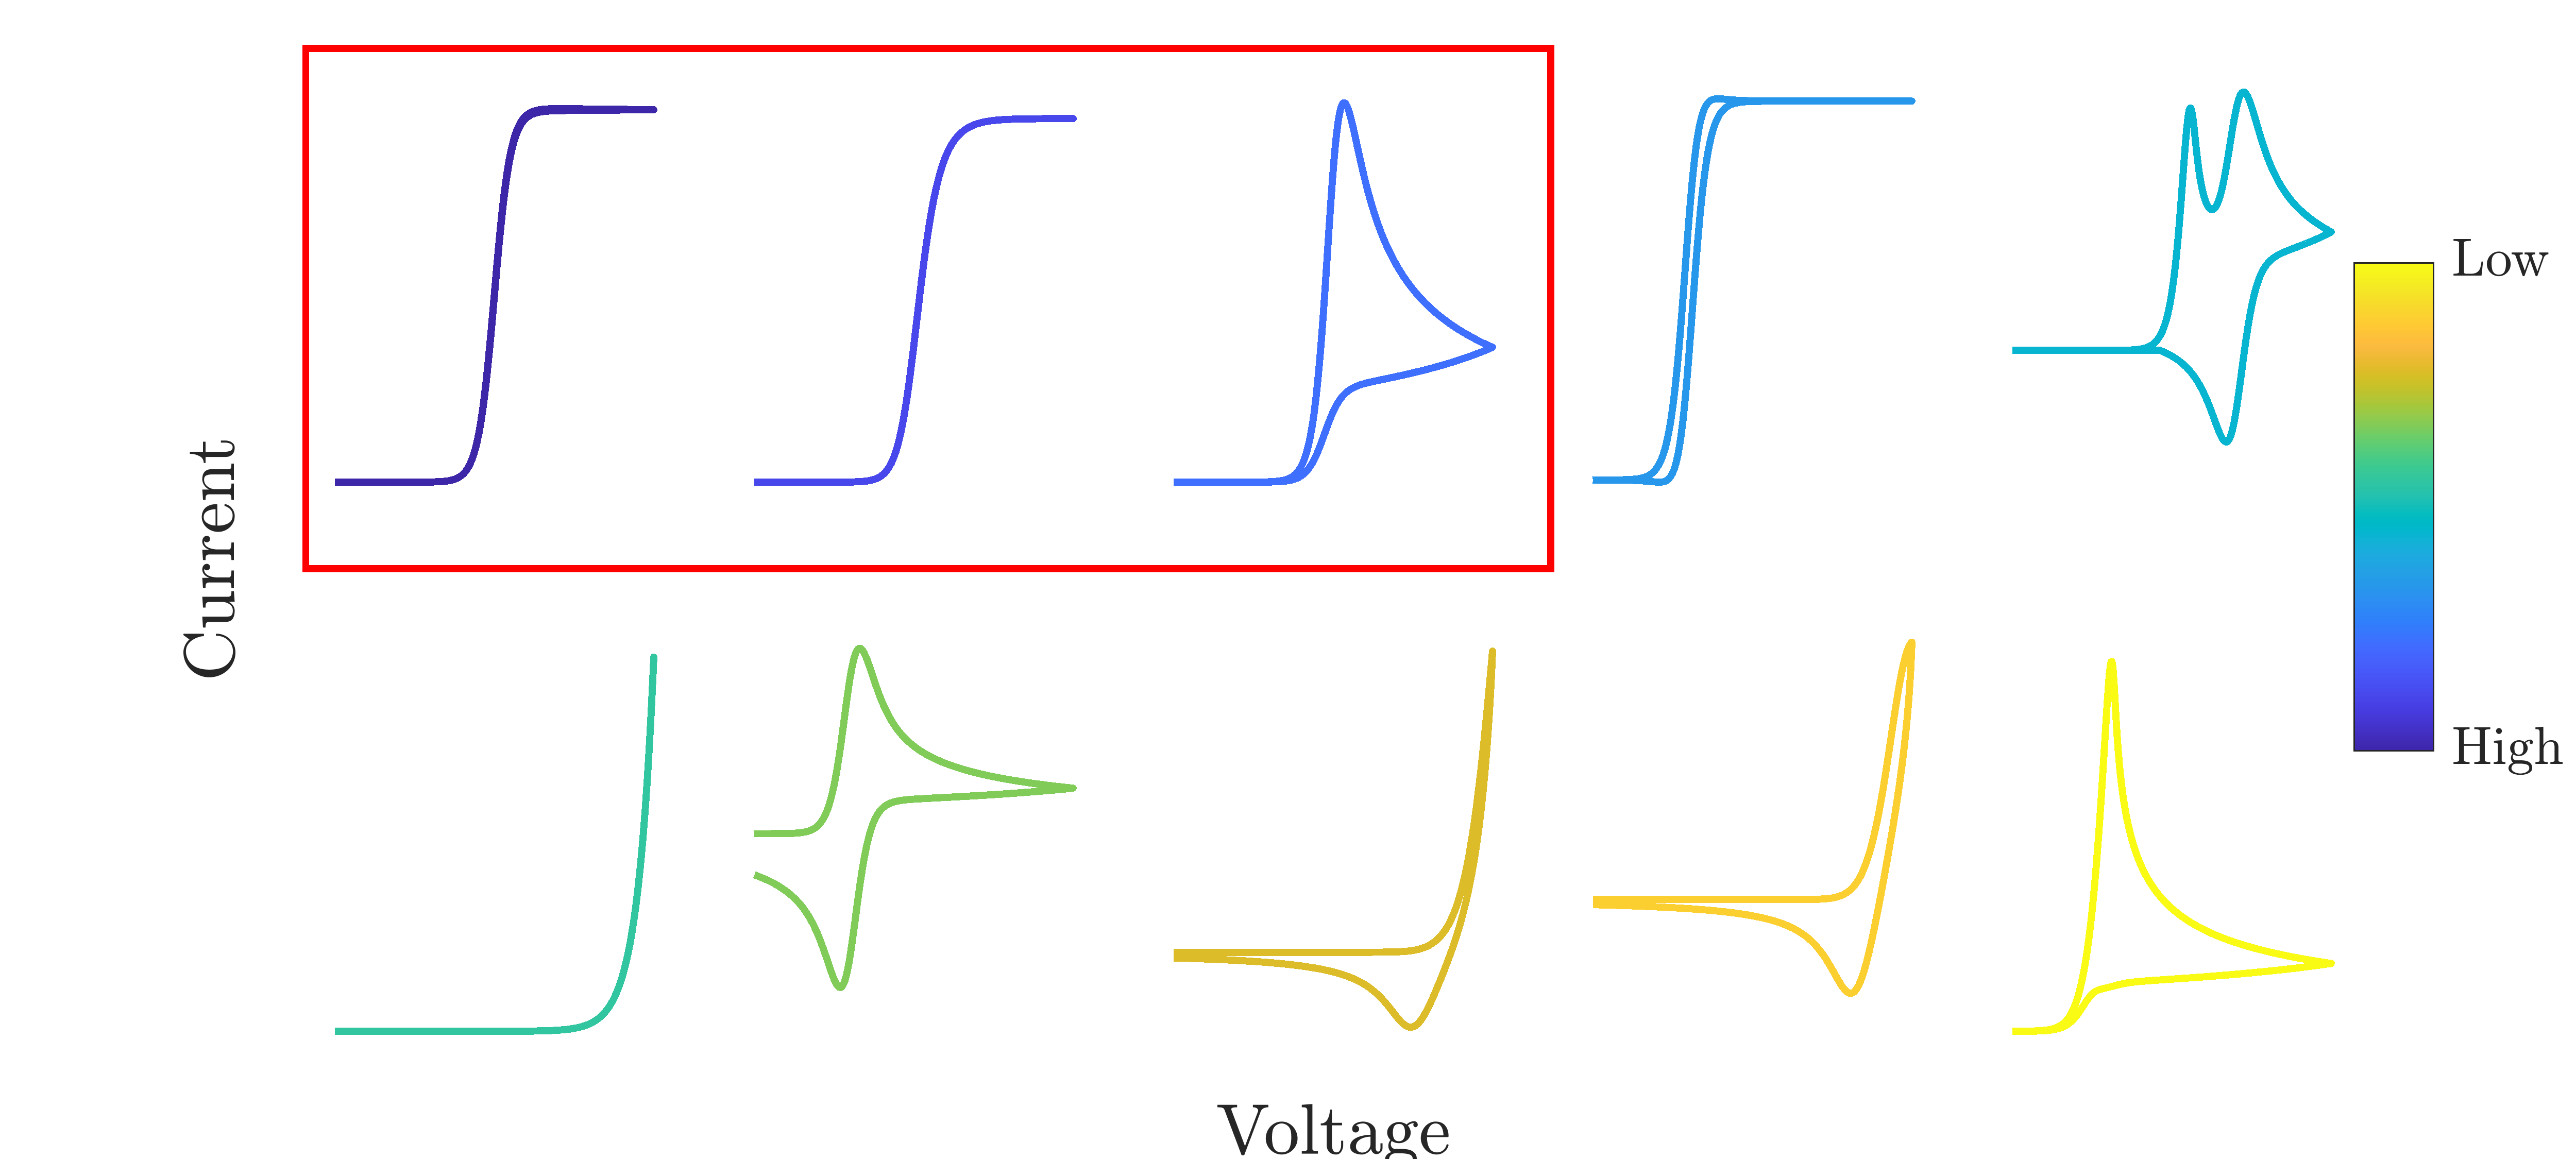
\includegraphics[width=100mm]{Chapter-3/figures/repsimscorespectrum.png}
    \caption{Representative CV curves from the dataset ordered and color coded using the similarity score. CV curves in the red box will be labelled as targets by the similarity score based oracle described here.}
    \label{figSI:repssscores}
\end{figure}

\subsubsection{FOWA-based score} 
In this subsection, a scoring method using the Foot of The Wave Analysis~(FOWA) ~\cite{costentin2015cyclic} is derived.
In the FOWA analysis, the original signal \((I,V)\) is transformed using the map \((I,V)\mapsto(I,1+\exp[\frac{F}{RT}(E-E^0)])\). 
An S-shaped CV curve is expected to be linear in two-dimensional FOWA coordinate space. 
Thus, a CV curve is scored based on its \(R^2\)-value computed with reference to user defined reference S-shape (for multiple S-shaped CV curves, maximum \(R^2\) value over the set is used), quantifying the linearity of the curve after the FOWA transformation.
~\Cref{figSI:repfowascores} is similar to~\Cref{fig:repbmsscores} with the rank of the curves determined by FOWA-based score. 
FOWA-based score ranks two of the target S-shaped CV curves in the top category. 
However, it fails to rank another S-shaped CV curve, like the fourth curve with a current onset only slightly shifted.
When discussing the effectiveness, we note that both of the approaches mentioned in this section depend on the usage of reference S-shapes from which the \(R^2\) value is computed. 
In particular, user needs to select a set of S-shapes that span the expected range in terms of current onset, rate constant etc., which is a non-trivial choice and adds to the heuristics. 
For these reasons BMS is preferred as it exploits the geometrical shape of CV curves directly without need for any user defined references. 
Moreover, note that BMS has an inherent ability to account for Gaussian noise. 
\begin{figure}[h]
    \centering
    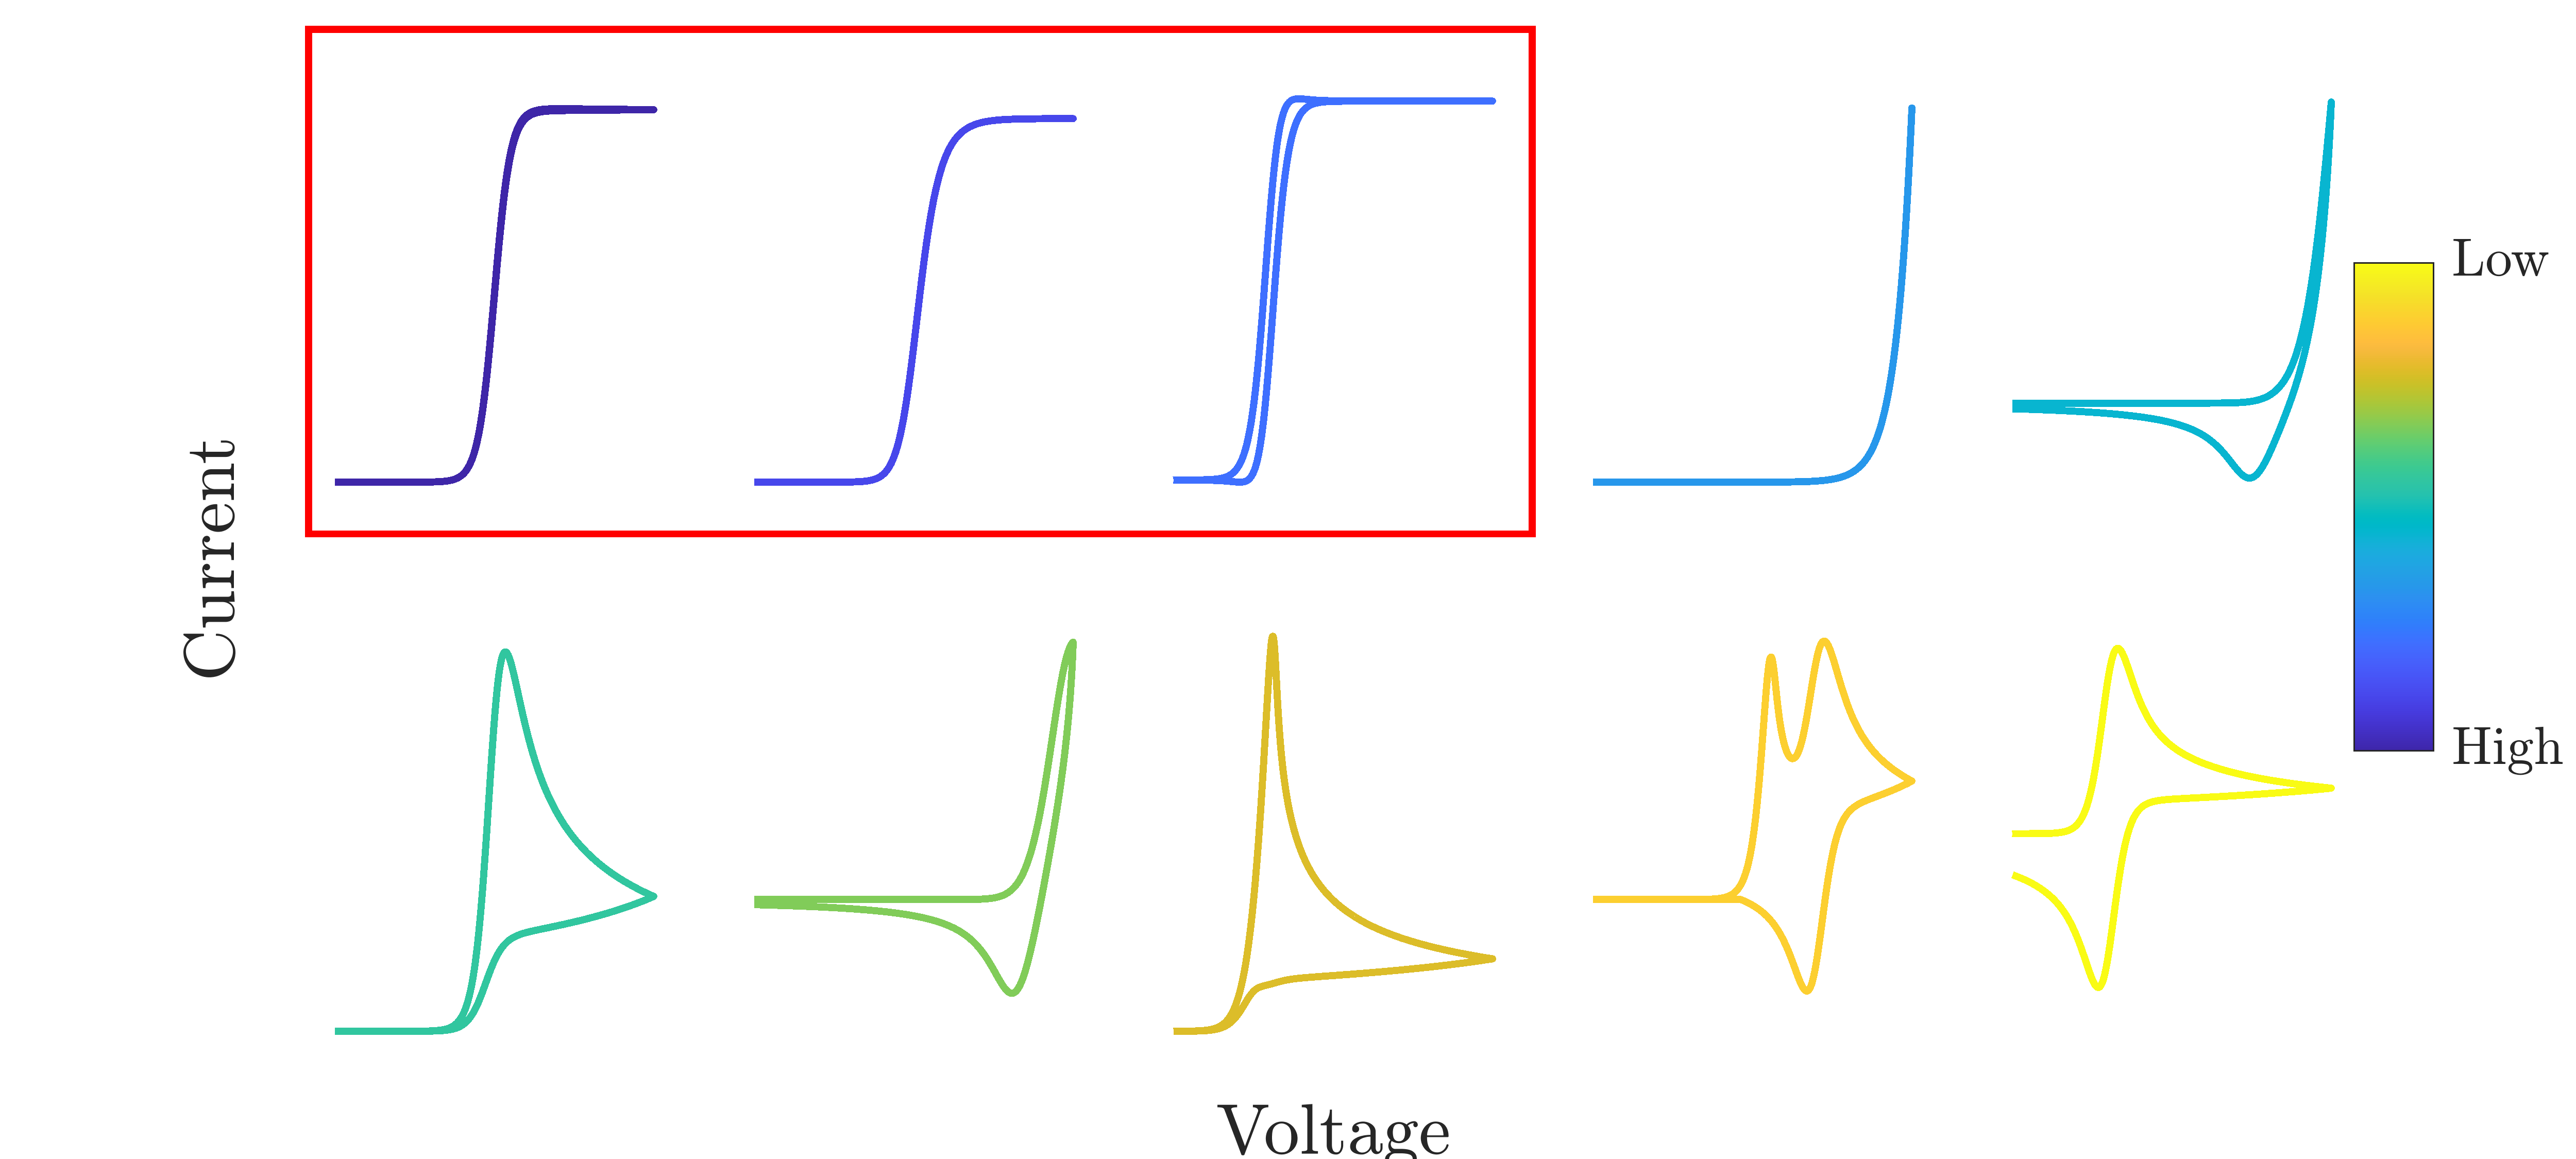
\includegraphics[width=100mm]{Chapter-3/figures/repfowaspectrum.png}
    \caption{Representative CV curves from the dataset ordered and color coded using the FOWA score. CV curves in the red box will be labelled as targets by the similarity FOWA score based oracle described here}
    \label{figSI:repfowascores}
\end{figure}

\section{Active (Batch)Search for S-shaped CV curves}
Active search with batch selection of locations in the design space has been recently studied and successfully applied to  high throughput combinatorial search of material and drug discovery~\cite{jiang2018efficient}. 
We use the state-of-the-art active batch search introduced in Jiang et.al~\cite{jiang2018efficient}, with a fixed budget of 1000 queries~(\(\approx6\%\) of exhaustive search over the grid \(\mathcal{S}\) in \Cref{tab:search_space}) to the simulator for batch sizes of \(b\in\{1,100\}\) to actively query our combinatorial search space~\(\mathcal{S}\).
The batch size reflects the setting of the high throughput analysis, as often material is prepared in batches.

A label for any given location is assigned based on the application of BMS oracle to the corresponding CV curve \(I(v,t)\) simulated by solving~\Cref{{eq:fickslaws,eq:bcs}} over \(4\times10^3\) discrete time points. 
A CV response is labelled as target if its BMS oracle score is in the range defined by top three percentile ranks~\footnote{this is a heuristic and can be altered based on application}~\footnote{Similarly for active search of bi-functional oxygen electrocatalysts, one can assign a material as a target if both of its OER and ORR experimental CV curves are in the top three percentile ranks of BMS scores. } shown in~\Cref{fig:repbmsscores}. 

\begin{figure}[h]
    \centering
    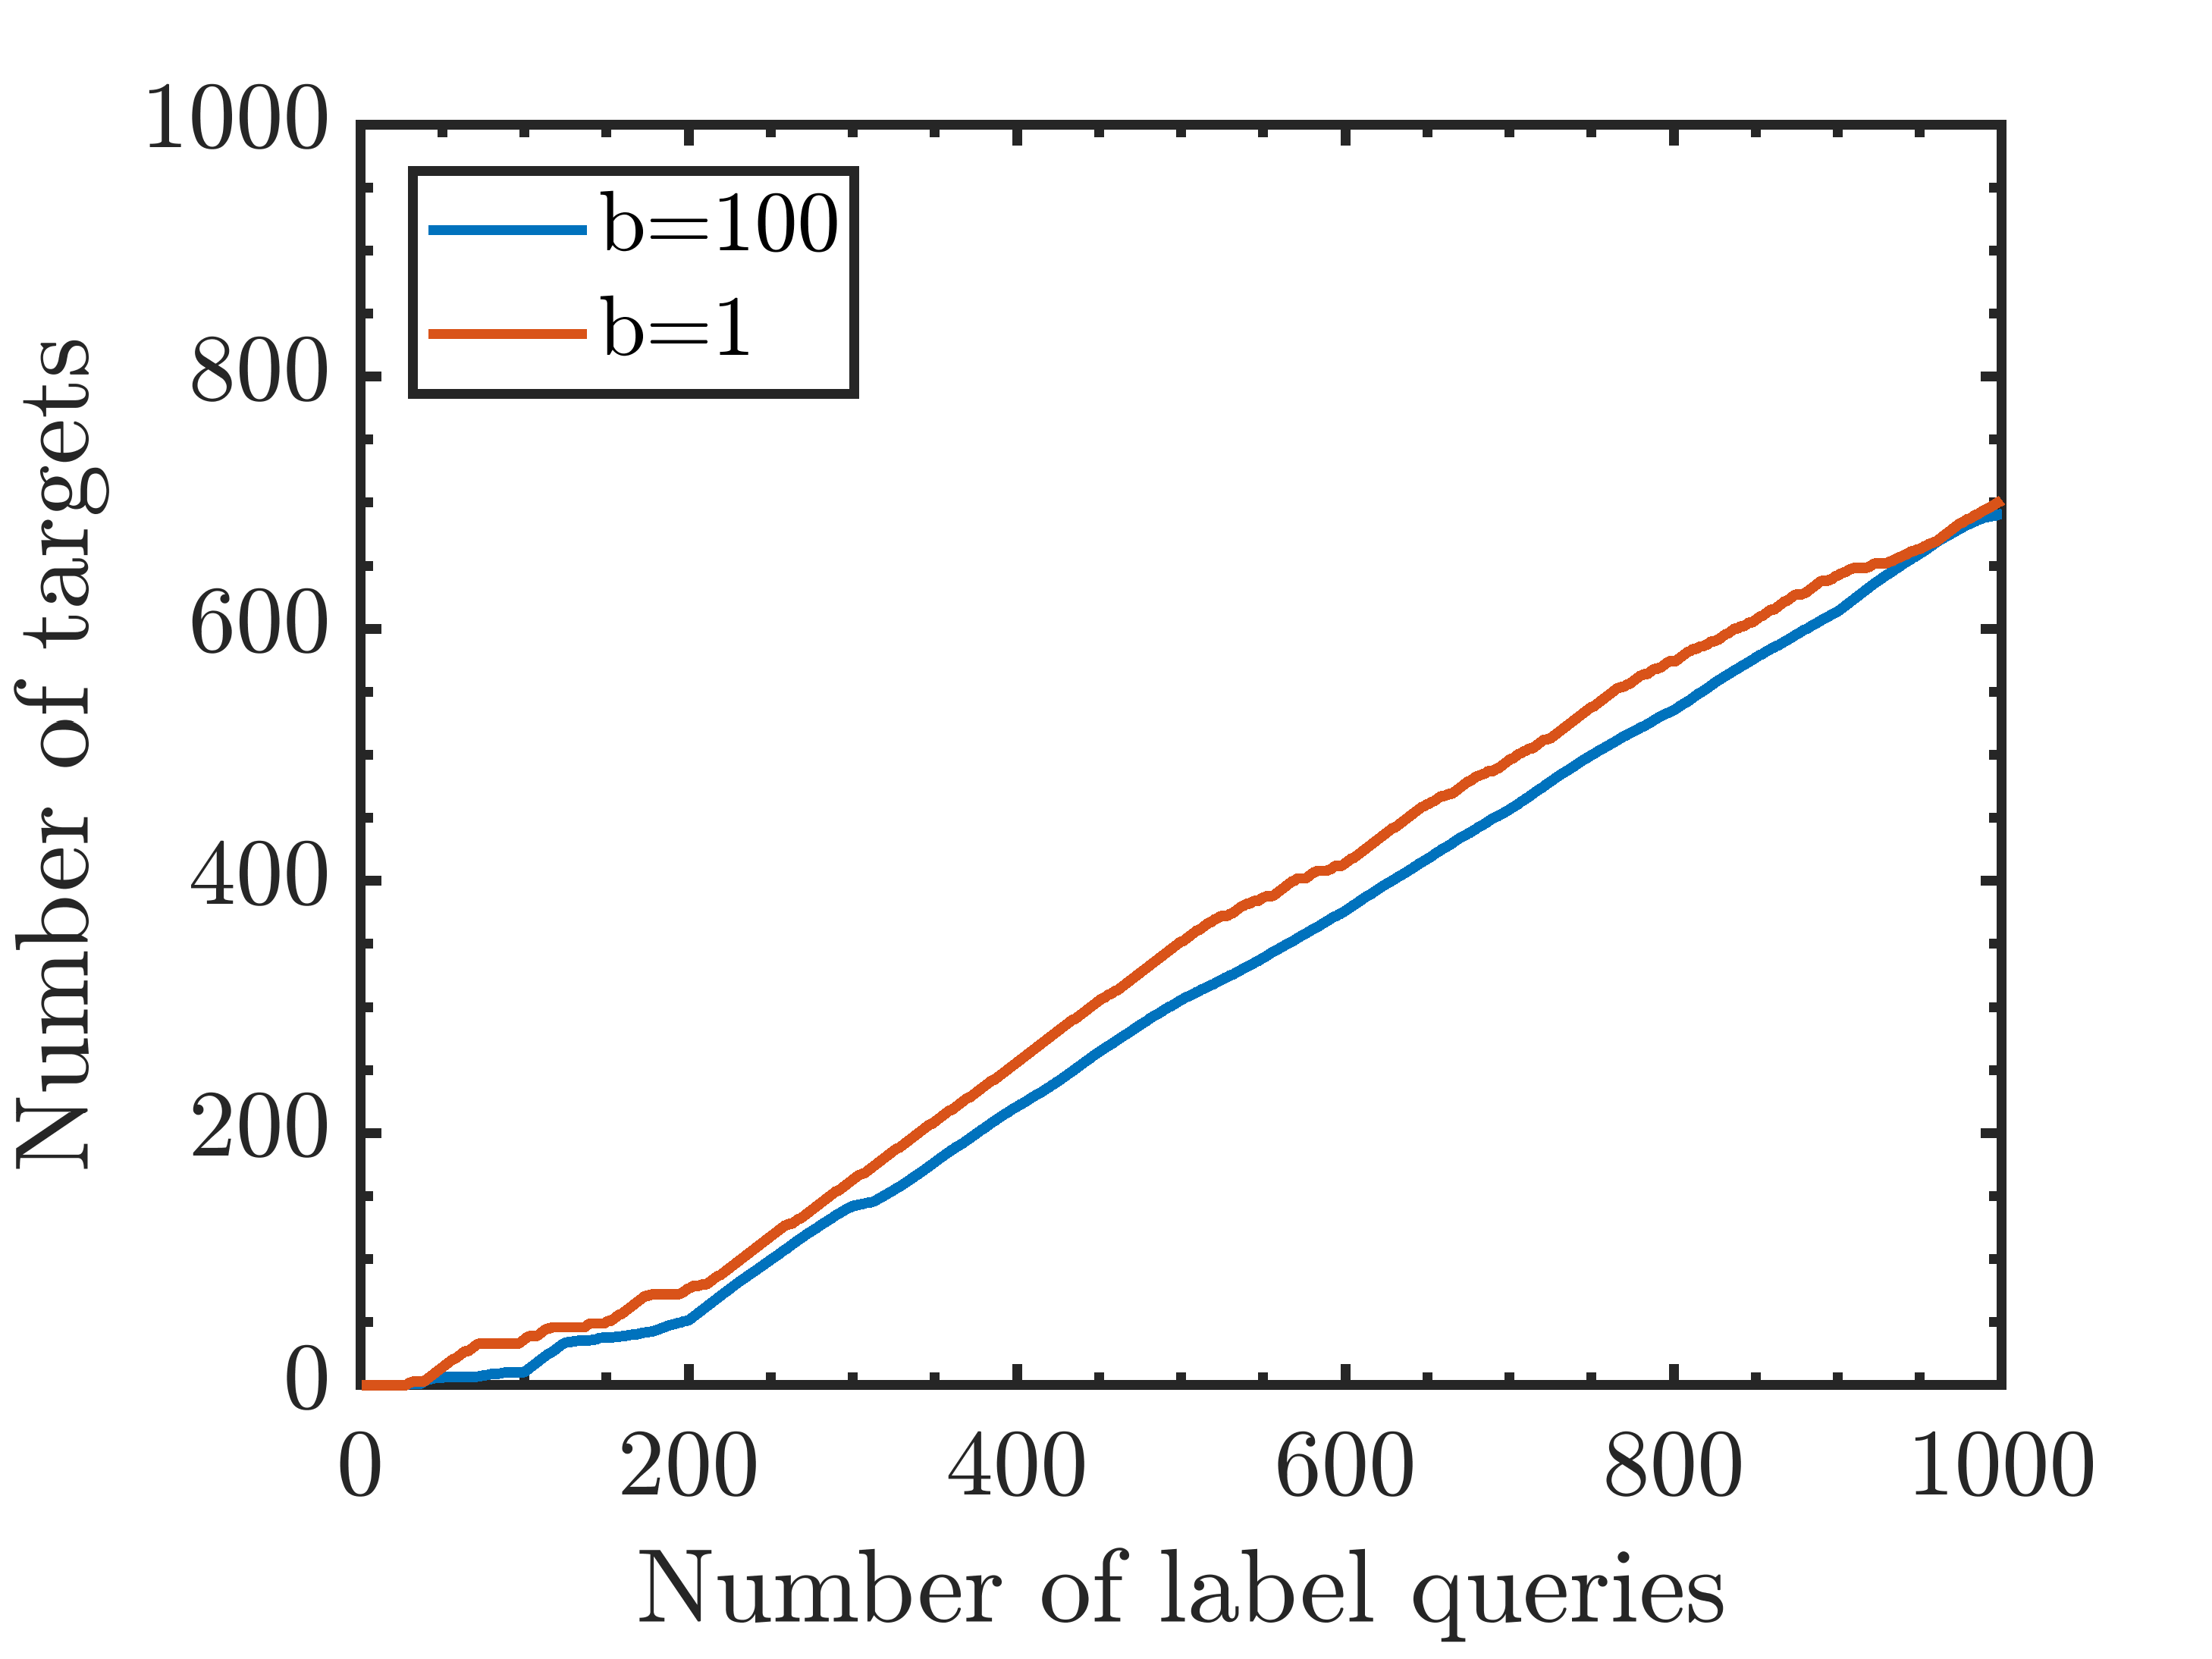
\includegraphics[width=100mm]{Chapter-3/figures/batch_results.png}
    \caption{Active target detection in the EC mechanism combinatorial search space (see~\Cref{tab:search_space} for definition of search space). We repeat the active search 20 times, each time starting with a randomly chosen non-S-shape data point in \(\mathcal{S}\). }
    \label{fig:batchens_fullec}
\end{figure}

Assuming that the design space is continuous, a \(k\)-nearest neighbor probability distribution is used a decision model in Bayesian active learning following the approach in~\cite{jiang2018efficient}. 
This assumption implies that if we find a target at a certain location in the search space, \(k\)-closest neighbors in the design space also are highly likely to be a target as well. 



In~\Cref{fig:batchens_fullec}, we report the average number of targets found in the design space over the number of label queries for two batch sizes \((b=1,100)\) considered~\footnote{The number of targets are averaged over a total of 20 active searches each time start with a randomly selected sample in the search space}.
Our results demonstrate that searching the design space using active learning can be useful, with a near linear target detection. 
It can also be noted from~\Cref{fig:batchens_fullec} for any given number of allowed label queries to the oracle~(or equivalently number of simulation queries to the simulator), the sequential selection finds marginally more targets than the batch selection \(b=100\).
This observation is in accordance with Theorem 1 in~\cite{jiang2018efficient}. 
Jiang et.al,~\cite{jiang2018efficient} argue that batch selection suffers from having to select a batch from the search space with fewer observed responses and locations. 
However, from experimental point of view, one need to consider the advantages and dis-advantages of sequential selection over batch selection. 


\section{Conclusion and future work}
In conclusion, \(\mathcal{GP}\)-based oracle is defined and evaluated for materials discovery using cyclic voltammetry.
Next, the oracle is combined with a state-of-the-art active batch search to identify conditions resulting in the targeted shape of CV curve. 
A robust high throughput combinatorial search is demonstrated to find the target responses using only \(<6\%\) of total number of CV experiments from the corresponding exhaustive search. 

As a future outlook, I anticipate that this work will have implications in identification of characterization conditions where kinetic knowledge extraction from the cyclic voltammetry can be preformed more effectively. 
Specifically, as illustrated using the active search framework, identification of S-shaped CV curves can lead to approximation rate constant of rate determining step. 
In this sense the framework discussed in this chapter has applications in accelerated knowledge extraction, with the application in screening for target catalysts including the bi-functional alkaline fuel cell catalysts that motivated this work.


